\documentclass[letter,11pt]{article}

\usepackage[spanish,es-nodecimaldot]{babel}
\usepackage[utf8]{inputenc}

\usepackage{lmodern}
\usepackage[T1]{fontenc}
\usepackage{textcomp}

\usepackage{framed}
\usepackage[svgnames]{xcolor}
\colorlet{shadecolor}{Gainsboro!50}

\usepackage[labelfont=bf]{caption}
\usepackage{graphicx}
\usepackage{pstricks}

\usepackage{anysize}
\marginsize{3cm}{2cm}{2cm}{3cm}

\usepackage{siunitx}
\usepackage{amsmath}
\usepackage{array}
\usepackage{alltt}

\usepackage{caption}
\newcommand{\source}[1]{\vspace{-11pt} \caption*{\small{\textbf{Nota:} {#1}}}}

\usepackage{fancyhdr}
\usepackage{lastpage}
\pagestyle{fancy}
\fancyhf{}
\fancyhead[LE,RO]{Laboratorio de Física Básica II}
\fancyfoot[CO,CE]{\thepage\ de \pageref{LastPage}}

\special{papersize=215.9mm,279.4mm}

\usepackage[
    pdfauthor={Carlos Eduardo Caballero Burgoa},%
    pdftitle={Laboratorio de Física Básica II},%
    pdfsubject={Módulo de elasticidad},%
    colorlinks,%
    citecolor=black,%
    filecolor=black,%
    linkcolor=black,%
    urlcolor=black,
    breaklinks]{hyperref}
\usepackage{breakurl}

\newcommand{\blankpage}{
\newpage
\thispagestyle{empty}
\mbox{}
\newpage
}

\renewcommand{\arraystretch}{1.2}

\title{Informe 1: Módulo de elasticidad}
\author{Carlos Eduardo Caballero Burgoa \\
    \small{\href{mailto:200201226@est.umss.edu}{200201226@est.umss.edu}}
}
\date{\today}

\begin{document}

\maketitle
\begin{center}
    \textbf{Grupo}: J2\\
    \textbf{Docente}: Ing. Milka Mónica Torrico Troche\\
    \textbf{Carrera}: Ing. Electromecánica
\end{center}

\begin{abstract}
Este documento detalla el experimento realizado para calcular el módulo de
elasticidad de una banda elástica, además de mostrar sus regiones de
comportamiento elástico, comportamiento plástico, y punto de ruptura; para esto
se realizó la medición de la elongación de la banda elástica a diferentes
cantidades de masa hasta el punto de ruptura; se tomo las mediciones realizadas
dentro de la zona elástica para hallar la recta de ajuste con el método de
mínimos cuadrados, y finalmente se determinó el valor del módulo de elasticidad
($Y$) resultando ser igual a: $(0.322 \pm 0.005)[MPa]; 1.48\%$.
\end{abstract}

\section{Introducción}

Todo objeto pueden ser sometido a varios tipos de fuerzas externas, ya sea el
estiramiento, la compresión, o la torcedura; la magnitud de estas deformaciones
y las fuerzas aplicadas, nos permiten determinar el comportamiento de los
materiales ante tales fuerzas.

Se denomina \textbf{esfuerzo} ($\sigma$) a la cantidad vectorial que representa
la intensidad de las fuerzas que causan el cambio de forma del objeto, mientras
que la medida de ese cambio se denomina \textbf{deformación} ($\epsilon$).

De la ley de \emph{Hooke}, se sabe que:

\begin{equation}
    \frac{\text{esfuerzo}}{\text{deformación}} = \text{constante}
\label{hooke}
\end{equation}
\vspace{0.10cm}

\begin{figure}
\centering
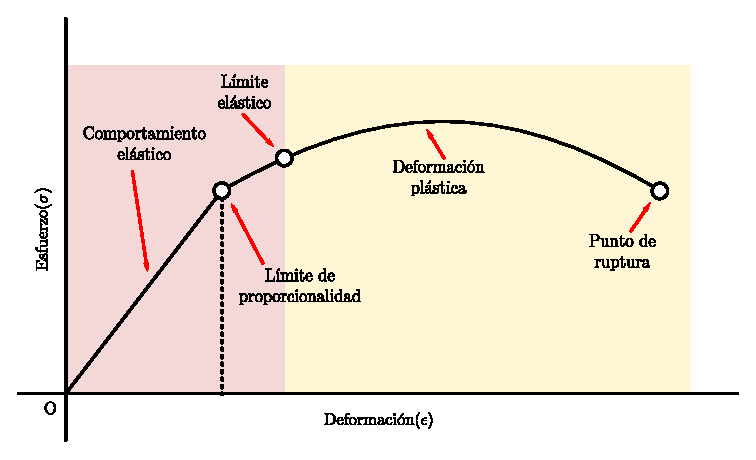
\includegraphics[width=0.80\textwidth]{resources/f1.eps}
\caption{Comportamiento del esfuerzo en función de la deformación.}
\label{figura1}
\source{Física Universitaria Volumen I (p. 358), \\
Young, Hugh D. y Freedman, Roger A., 2013, Pearson.}
\end{figure}

Esta ley es solo aplicable a deformaciones unitarias pequeñas, hasta alcanzar
el limite de proporcionalidad del material, como puede verse en la
\textbf{Figura \ref{figura1}}.

En las curvas esfuerzo vs. deformación de un material hay un tramo de
comportamiento perfectamente elástico en el que la relación es lineal (hasta el
limite de proporcionalidad). De ahí hasta el límite elástico, el material sigue
un comportamiento elástico (existe una relación entre esfuerzo y deformación,
aunque no es lineal, y si se retira el esfuerzo se recupera la
longitud inicial). Si se sigue aumentando la carga (por encima de ese punto), el
material se deforma rápidamente y si se retira el esfuerzo no se recupera la
longitud inicial, quedando una deformación permanente y el cuerpo tiene un
comportamiento plástico. Si se sigue aumentando la carga, el material llega
hasta un estado en el que se rompe (punto de ruptura) \cite{Young&Freedman}.

Dentro del limite elástico (donde la ley de \emph{Hooke} es valida), se halla
esa constante propia del material con la siguiente ecuación:

\begin{equation}
    Y = \frac{\sigma}{\epsilon}
\label{young1}
\end{equation}
\vspace{0.10cm}

Donde: $\sigma$ es el esfuerzo, y $\epsilon$ es la deformación unitaria (en este
caso longitudinal) para una banda elástica.

Para el calculo del esfuerzo ($\sigma$) se usa la siguiente ecuación:

\begin{equation}
    \sigma = \frac{F_{\perp}}{A}
\label{sigma}
\end{equation}
\vspace{0.10cm}

Donde: $F_{\perp}$ es la magnitud de la fuerza de tensión realizada
perpendicular al área transversal, y $A$ el área de tal sección transversal del
material.

Mientras que para calcular la deformación unitaria ($\epsilon$) se tiene la
siguiente ecuación:

\begin{equation}
    \epsilon = \frac{l - l_o}{l_o} = \frac{\Delta l}{l_o}
\label{epsilon}
\end{equation}
\vspace{0.10cm}

Donde: $\Delta l$ es la diferencia entre la longitud inicial ($l_o$) del
material y la longitud actual ($l$).

Reemplazando $\sigma$ de la \textbf{Ecuación \ref{sigma}} y $\epsilon$ de la
\textbf{Ecuación \ref{epsilon}}, en la \textbf{Ecuación \ref{young1}}
\cite{GUIA}, se obtiene:

\begin{equation}
    \frac{F}{A} = Y\,\frac{\Delta l}{l_o}
\label{young2}
\end{equation}
\vspace{0.10cm}

Para el experimento se tomará los datos del estiramiento de la banda elástica
($l$) a diferentes masas de carga ($m$), y hasta alcanzar el punto de ruptura;
luego se realizará la gráfica esfuerzo vs. deformación unitaria para una
deformación longitudinal por tensión, de forma que pueda apreciarse las
diferentes etapas de su comportamiento.

También se hallará la relación funcional del esfuerzo vs. deformación unitaria,
y finalmente se hallará el módulo de elasticidad del material.

\section{Método experimental}

\begin{figure}
\centering
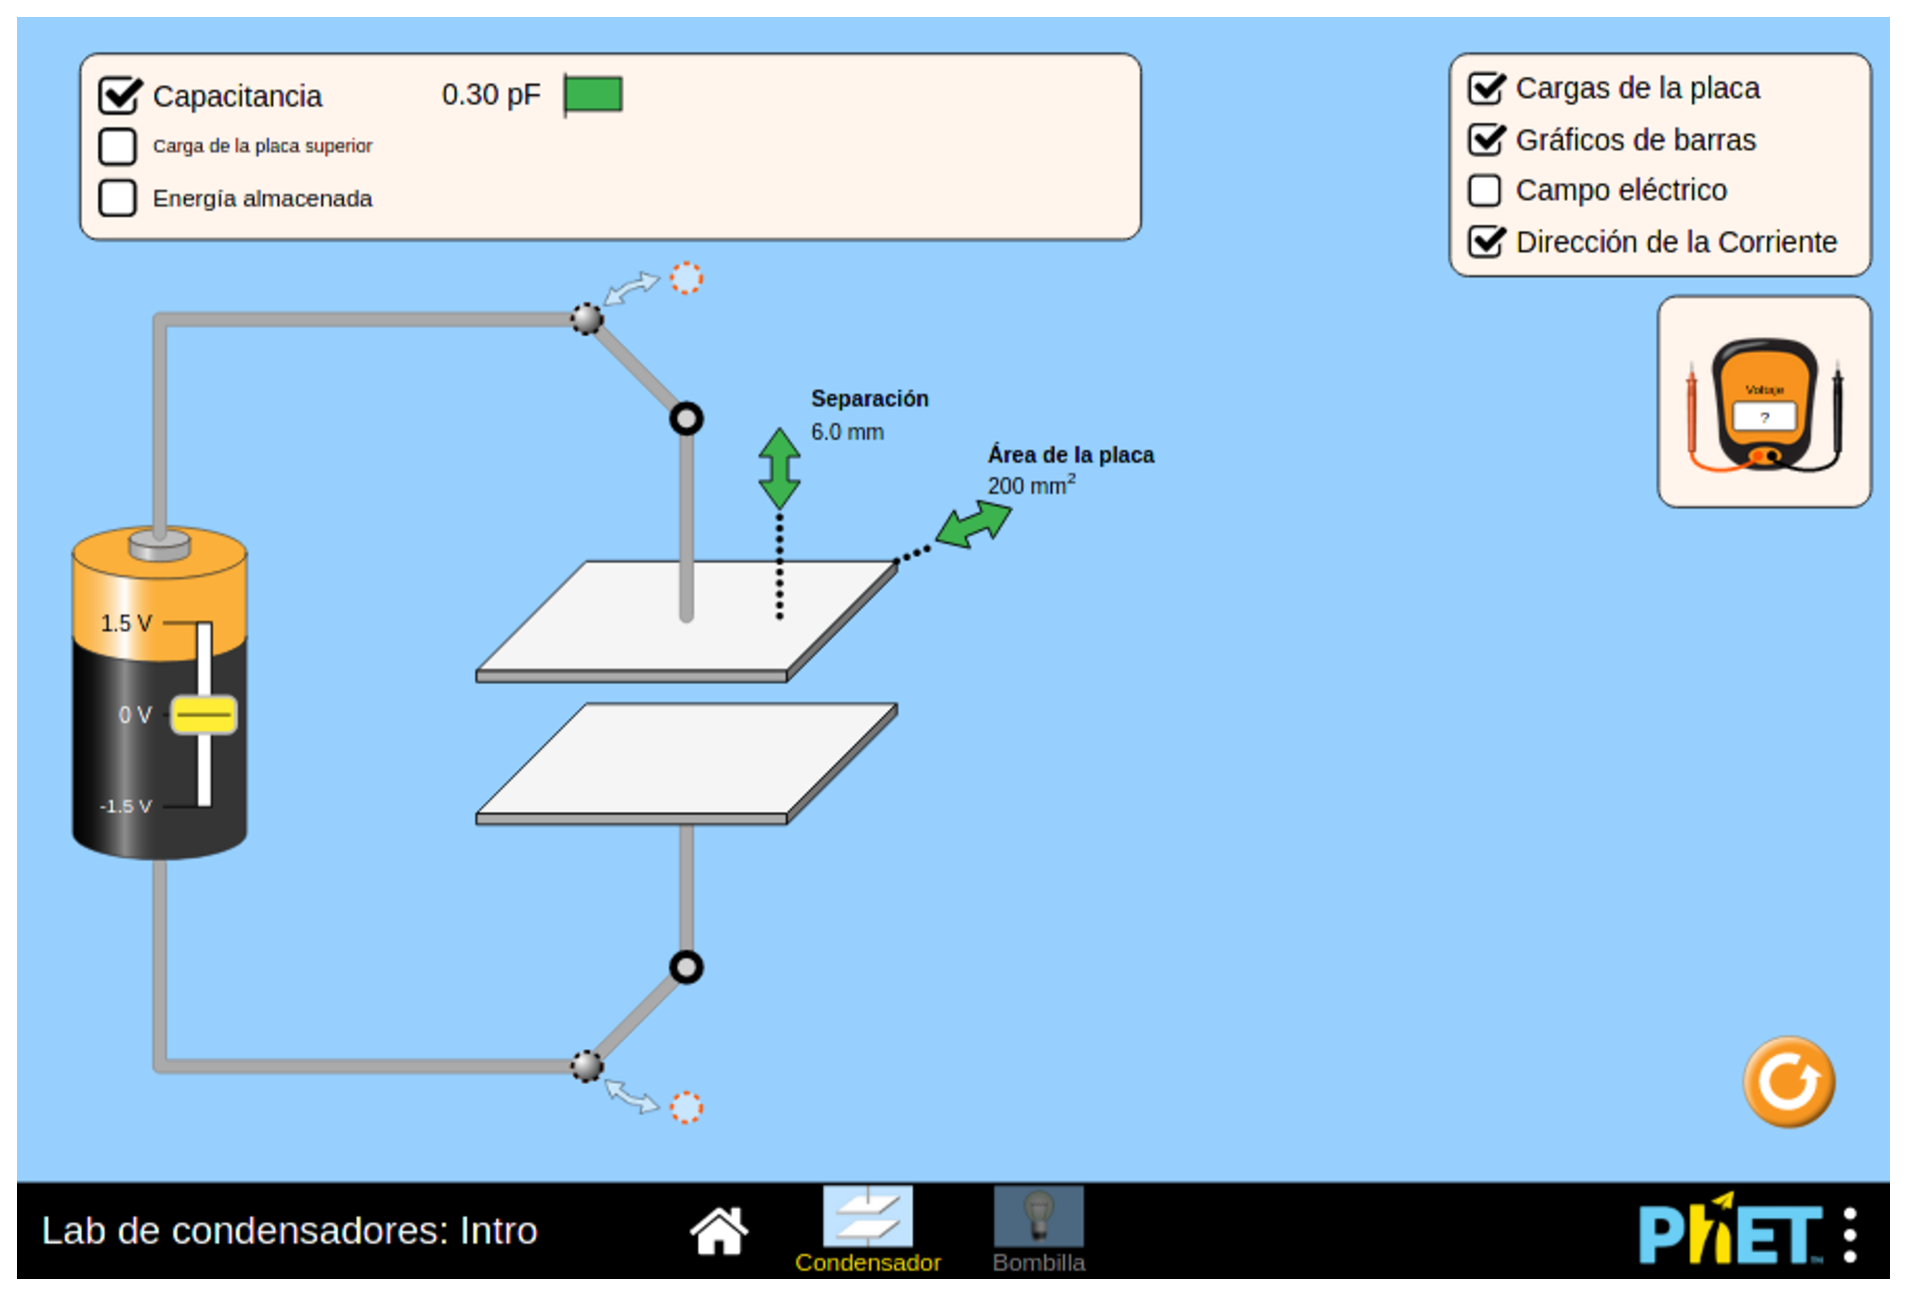
\includegraphics[width=0.65\textwidth]{resources/f3.eps}
\caption{Montaje del experimento.}
\label{figura2}
\source{Fotografía propia.}
\end{figure}

Para facilitar la medición, se ha armado el equipo mostrado en la
\textbf{Figura \ref{figura2}}, el cual consta de un \textbf{trípode},
previamente nivelado, y una \textbf{regla de 60 centímetros} (Precisión:
$1 [mm]$) para facilitar la medición.

Al trípode se ha sujetado la \textbf{banda elástica}, suspendiendo de esta un
contenedor vacío previamente pesado en una \textbf{balanza} (Precisión:
$0.1 [g]$).

Una vez montado el soporte, se midió el área de la banda elástica con ayuda de
un \textbf{calibrador} (Precisión: $0.1 [mm]$).

\begin{figure}
\centering
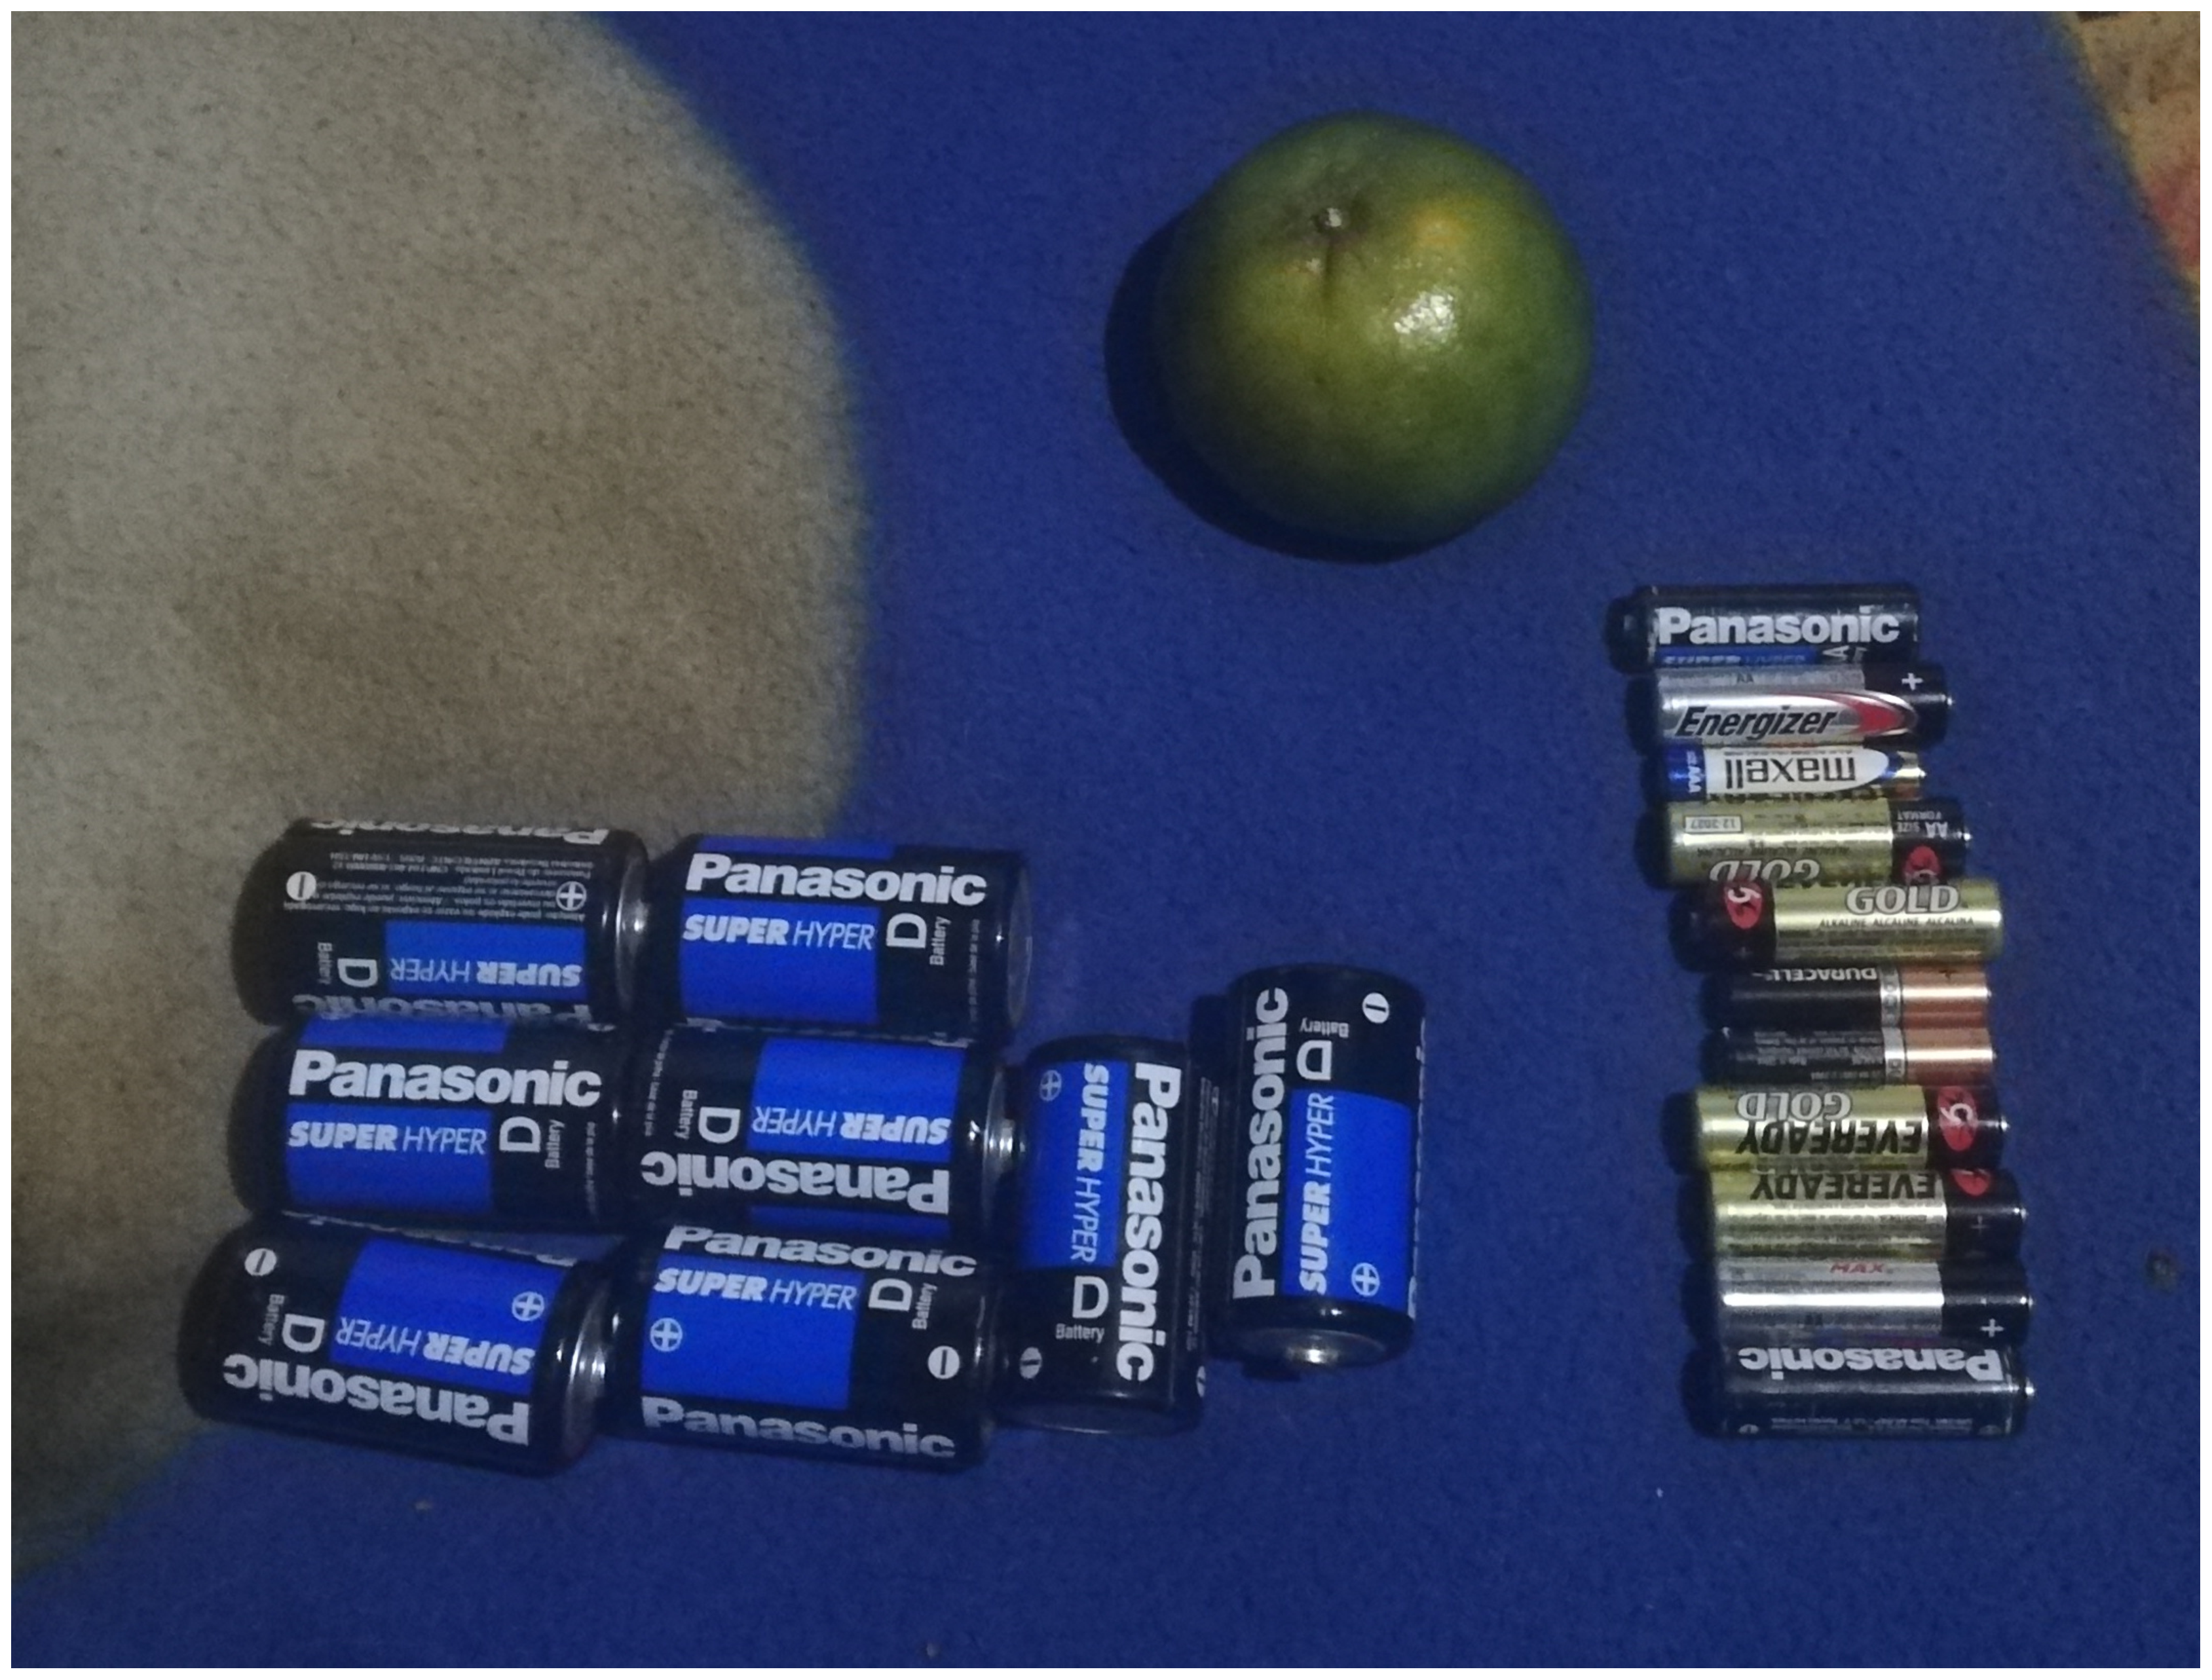
\includegraphics[width=0.65\textwidth]{resources/f2.eps}
\caption{Conjunto de pesos a utilizar.}
\label{figura3}
\source{Fotografía propia.}
\end{figure}

Posteriormente se midió la longitud inicial de la banda elástica ya suspendida;
y se procedió a agregar masa ($m$) al contenedor, a partir de un
\textbf{conjunto de pesos} (en este caso baterías \emph{A}, \emph{AA}, y
\emph{AAA}) como los mostrados en la \textbf{Figura \ref{figura3}}.

Se registró el incremento de la longitud, hasta alcanzar el punto de ruptura de
la banda elástica.

\vspace{0.35cm}
\textbf{Datos necesarios para el experimento:} \\

Aceleración de la gravedad local:

\begin{equation*}
    g = (9.78 \pm 0.02)[m/s^2]
\end{equation*}
\vspace{0.10cm}

Masa del contenedor vacío:

\begin{equation*}
    m = (40.8 \pm 0.1)[g]
\end{equation*}
\vspace{0.10cm}

Dimensiones de la banda elástica:

\begin{equation*}
    a_1 = (2.0 \pm 0.1)[mm]
\end{equation*}
\begin{equation*}
    a_2 = (1.6 \pm 0.1)[mm]
\end{equation*}
\vspace{0.10cm}

Área transversal de la banda elástica:

\begin{equation*}
    A = (\num{3.2e-6} \pm \num{2.56e-7})[m^2]
\end{equation*}
\vspace{0.10cm}

Longitud inicial de la banda elástica:

\begin{equation*}
    L_o = (0.041 \pm 0.001)[m]
\end{equation*}

\vspace{0.35cm}
\textbf{Datos tomados en el experimento:} \\

En el \textbf{cuadro \ref{cuadro1}}, pueden ver los valores tomados del 
experimento, tanto la masa como la longitud de la deformación resultante:

\begin{table}[!h]
\begin{center}
\begin{tabular}{|c||>{\centering}m{1.5cm}<{\centering}
                   |>{\centering}m{1.5cm}<{\centering}|
                |c||>{\centering}m{1.5cm}<{\centering}
                   |>{\centering}m{1.5cm}<{\centering}|}
\hline
$i$ & $m_i [g]$ & $l_i [cm]$ & $i$ & $m_i [g]$ & $l_i [cm]$
    \tabularnewline \hline \hline
 1 &    0   &  4.1 & 23 &  512.5 & 20.6 \tabularnewline \hline
 2 &   23.4 &  4.6 & 24 &  535.9 & 21.3 \tabularnewline \hline
 3 &   46.9 &  5.5 & 25 &  559.4 & 22.5 \tabularnewline \hline
 4 &   70.0 &  6.4 & 26 &  583.0 & 23.2 \tabularnewline \hline
 5 &   93.1 &  7.5 & 27 &  606.2 & 24.2 \tabularnewline \hline
 6 &  116.4 &  7.9 & 28 &  623.4 & 24.7 \tabularnewline \hline
 7 &  139.6 &  8.9 & 29 &  640.7 & 25.0 \tabularnewline \hline
 8 &  162.9 &  9.8 & 30 &  658.3 & 25.4 \tabularnewline \hline
 9 &  185.7 & 10.8 & 31 &  674.8 & 25.5 \tabularnewline \hline
10 &  207.8 & 11.6 & 32 &  697.1 & 25.8 \tabularnewline \hline
11 &  231.1 & 12.7 & 33 &  733.5 & 26.5 \tabularnewline \hline
12 &  254.4 & 13.5 & 34 &  769.4 & 27.7 \tabularnewline \hline
13 &  277.6 & 14.6 & 35 &  802.3 & 28.0 \tabularnewline \hline
14 &  301.0 & 15.8 & 36 &  837.0 & 29.0 \tabularnewline \hline
15 &  324.3 & 16.2 & 37 &  862.3 & 29.1 \tabularnewline \hline
16 &  347.5 & 17.1 & 38 &  898.2 & 29.5 \tabularnewline \hline
17 &  370.3 & 17.8 & 39 &  932.2 & 29.8 \tabularnewline \hline
18 &  393.6 & 18.1 & 40 &  965.6 & 30.5 \tabularnewline \hline
19 &  420.1 & 19.1 & 41 & 1007.2 & 30.8 \tabularnewline \hline
20 &  443.2 & 19.3 & 42 & 1046.0 & 31.3 \tabularnewline \hline
21 &  466.7 & 19.7 & 43 & 1085.2 & 31.8 \tabularnewline \hline
22 &  489.8 & 20.3 & 44 & 1126.3 & 32.3 \tabularnewline \hline
\end{tabular}
\caption{Mediciones de longitud en función de la masa provista.}
\label{cuadro1}
\source{Elaboración propia.}
\end{center}
\end{table}

\section{Resultados}

\begin{figure}
\centering
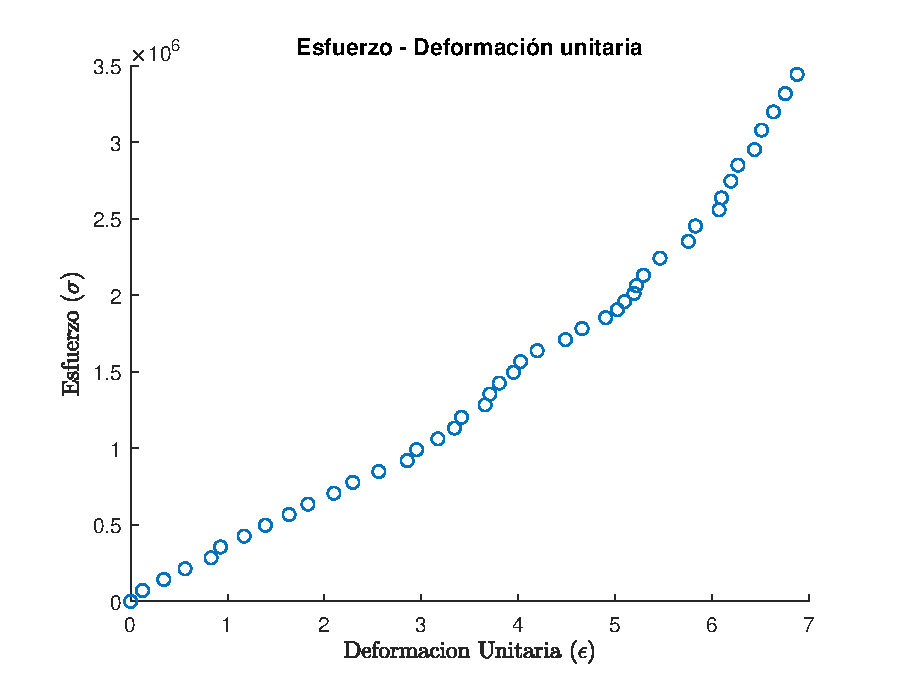
\includegraphics[width=0.80\textwidth]{resources/m1.eps}
\caption{Valores del esfuerzo y la deformación unitaria.}
\label{figura4}
\source{Elaboración propia.}
\end{figure}

A partir de los datos obtenidos se genera la gráfica de la
\textbf{Figura \ref{figura4}} del comportamiento del esfuerzo ($\sigma$) en
función a la deformación unitaria ($\epsilon$). Puede verse que el limite de
proporcionalidad es próximo al valor de 3 unidades de deformación unitaria.

Posteriormente se calculo la recta de mejor ajuste por el método de los mínimos
cuadrados tomando las primeras 15 mediciones, resultando los siguientes valores:

\begin{equation*}
    A = (\num{3.24e4} \pm \num{8.19e3}) [N/m^2]; 25.24\%
\end{equation*}
\begin{equation*}
    B = (\num{3.22e5} \pm \num{4.76e3}) [N/m^2]; 1.47\%
\end{equation*}
\vspace{0.10cm}

Siendo su coeficiente de correlación ($r$):
\begin{equation*}
    r = 0.9986
\end{equation*}
\vspace{0.10cm}

Considerando que el modelo de ajuste es:

\begin{equation*}
    \sigma = A + B \epsilon
\end{equation*}
\vspace{0.10cm}

Por tanto la relación funcional entre $\sigma$ y $\epsilon$, es:

\begin{equation*}
    \sigma \propto \epsilon
\end{equation*}
\vspace{0.10cm}

El módulo de elasticidad para la banda elástica del experimento es:

\begin{equation*}
    Y = (\num{3.22e5} \pm \num{4.76e3}) [N/m^2]; 1.48\%
\end{equation*}
\vspace{0.10cm}

Convirtiendo a $MPa$, se obtiene:

\begin{equation*}
    Y = (0.322 \pm 0.005) [MPa]; 1.48\%
\end{equation*}

\section{Discusión}

Si bien los datos obtenidos reflejan claramente las zonas de comportamiento del
material, se debe destacar lo complicado que es agregar masa mientras la banda
elástica se encuentra en la zona plástica, ya que esta comienza a estirarse sin
necesidad de masa adicional, por lo cual las mediciones en esta zona sean muy
imprecisas.

Tuvieron que hacerse tres pruebas antes de la toma de datos, para determinar la
cantidad apropiada de masa a ir agregando de forma que se obtengan suficientes
datos en la zona elástica.

Finalmente al no contar con tantos pesos similares, se tuvieron que realizar
equivalencias de peso para mantener los incrementos de masa constantes, lo que
podría afectar ligeramente las mediciones, dependiendo de la zona en la que este
el material.

Por tal motivo, debe considerarse que el incremento de masa mas apropiado seria
aquel que puede dividirse a grado muy fino, por ejemplo: la arena, o granos de
arroz, de esa forma el control sobre el incremento de masa seria total.

\section{Conclusiones}

Se realizó la gráfica de esfuerzo vs deformación unitaria, en esta puede
apreciarse tanto la zona elástica, como la zona plástica.

Se realizó el ajuste de la recta por el método de mínimos cuadrados y se halló
la relación funcional entre estas dos variables, siendo está constante el
módulo de elasticidad.

\begin{thebibliography}{99}

\bibitem{Young&Freedman} Young, Hugh D. y Freedman, Roger A. (2013).\\
Física Universitaria. Volumen 1.\\
13va Edición.\\
Capitulo 11.

\bibitem{GUIA} Departamento de Física - UMSS.\\
Laboratorio de Física Básica II.\\
Guía - Cartilla de laboratorio.\\
Gestión I/2020.

\end{thebibliography}

\newpage
\section*{Apéndice: Cálculos adicionales}

Conociendo $l$, $l_o$, $m$, $g$, y $A$, se detallan los valores del esfuerzo
($\sigma$) y la deformación unitaria ($\epsilon$) en el
\textbf{cuadro \ref{cuadro2}}.

\begin{table}[!h]
\begin{center}
\begin{tabular}{|c||>{\centering}m{2.8cm}<{\centering}
                   |>{\centering}m{1.8cm}<{\centering}|
                |c||>{\centering}m{2.8cm}<{\centering}
                   |>{\centering}m{1.8cm}<{\centering}|}
\hline
    $i$ & $\sigma_i [N/m^2] \num{e6}$ & $\epsilon_i$ &
    $i$ & $\sigma_i [N/m^2] \num{e6}$ & $\epsilon_i$ \tabularnewline \hline
\hline
 1 &      0 &      0 & 23 & 1.5663 & 4.0244 \tabularnewline \hline
 2 & 0.0715 & 0.1220 & 24 & 1.6378 & 4.1951 \tabularnewline \hline
 3 & 0.1433 & 0.3415 & 25 & 1.7097 & 4.4878 \tabularnewline \hline
 4 & 0.2139 & 0.5610 & 26 & 1.7818 & 4.6585 \tabularnewline \hline
 5 & 0.2845 & 0.8293 & 27 & 1.8527 & 4.9024 \tabularnewline \hline
 6 & 0.3557 & 0.9268 & 28 & 1.9053 & 5.0244 \tabularnewline \hline
 7 & 0.4267 & 1.1707 & 29 & 1.9581 & 5.0976 \tabularnewline \hline
 8 & 0.4979 & 1.3902 & 30 & 2.0119 & 5.1951 \tabularnewline \hline
 9 & 0.5675 & 1.6341 & 31 & 2.0624 & 5.2195 \tabularnewline \hline
10 & 0.6351 & 1.8293 & 32 & 2.1305 & 5.2927 \tabularnewline \hline
11 & 0.7063 & 2.0976 & 33 & 2.2418 & 5.4634 \tabularnewline \hline
12 & 0.7775 & 2.2927 & 34 & 2.3515 & 5.7561 \tabularnewline \hline
13 & 0.8484 & 2.5610 & 35 & 2.4520 & 5.8293 \tabularnewline \hline
14 & 0.9199 & 2.8537 & 36 & 2.5581 & 6.0732 \tabularnewline \hline
15 & 0.9911 & 2.9512 & 37 & 2.6354 & 6.0976 \tabularnewline \hline
16 & 1.0620 & 3.1707 & 38 & 2.7451 & 6.1951 \tabularnewline \hline
17 & 1.1317 & 3.3415 & 39 & 2.8490 & 6.2683 \tabularnewline \hline
18 & 1.2029 & 3.4146 & 40 & 2.9511 & 6.4390 \tabularnewline \hline
19 & 1.2839 & 3.6585 & 41 & 3.0783 & 6.5122 \tabularnewline \hline
20 & 1.3545 & 3.7073 & 42 & 3.1968 & 6.6341 \tabularnewline \hline
21 & 1.4264 & 3.8049 & 43 & 3.3166 & 6.7561 \tabularnewline \hline
22 & 1.4970 & 3.9512 & 44 & 3.4423 & 6.8780 \tabularnewline \hline
\end{tabular}
\caption{Calculo del esfuerzo y la deformación unitaria.}
\label{cuadro2}
\source{Elaboración propia.}
\end{center}
\end{table}

Se calculan los parámetros de la recta por el método de los mínimos cuadrados,
con la ayuda de los datos presentados en el \textbf{Cuadro \ref{cuadro3}}.

\begin{table}[!h]
\begin{center}
\begin{tabular}{|c||>{\centering}m{1.6cm}<{\centering}
                   |>{\centering}m{1.6cm}<{\centering}
                   |>{\centering}m{1.6cm}<{\centering}|
                   |>{\centering}m{1.6cm}<{\centering}
                   |>{\centering}m{1.6cm}<{\centering}
                   |>{\centering}m{1.6cm}<{\centering}|}
\hline
$i$ & $x_i y_i (\num{e6})$ & $x^2_i$ & $y^2_i (\num{e11})$ &
    $Y_i (\num{e5})$ & $d_i (\num{e4})$ & $d^2_i\,(\num{e9})$
    \tabularnewline \hline \hline
 1 &      0 &      0 &      0 & 0.3243 & -3.2430 & 1.0517 \tabularnewline \hline
 2 & 0.0087 & 0.0149 & 0.0511 & 0.7176 & -0.0241 & 0.0001 \tabularnewline \hline
 3 & 0.0489 & 0.1166 & 0.2055 & 1.4255 &  0.0792 & 0.0006 \tabularnewline \hline
 4 & 0.1200 & 0.3147 & 0.4577 & 2.1334 &  0.0602 & 0.0004 \tabularnewline \hline
 5 & 0.2360 & 0.6877 & 0.8096 & 2.9986 & -1.5319 & 0.2347 \tabularnewline \hline
 6 & 0.3297 & 0.8590 & 1.2656 & 3.3132 &  2.4430 & 0.5968 \tabularnewline \hline
 7 & 0.4995 & 1.3706 & 1.8203 & 4.0997 &  1.6680 & 0.2782 \tabularnewline \hline
 8 & 0.6922 & 1.9328 & 2.4787 & 4.8076 &  1.7101 & 0.2925 \tabularnewline \hline
 9 & 0.9275 & 2.6704 & 3.2211 & 5.5942 &  0.8129 & 0.0661 \tabularnewline \hline
10 & 1.1617 & 3.3462 & 4.0334 & 6.2234 &  1.2749 & 0.1625 \tabularnewline \hline
11 & 1.4815 & 4.3998 & 4.9886 & 7.0886 & -0.2561 & 0.0066 \tabularnewline \hline
12 & 1.7826 & 5.2564 & 6.0452 & 7.7178 &  0.5726 & 0.0328 \tabularnewline \hline
13 & 2.1728 & 6.5586 & 7.1981 & 8.5830 & -0.9889 & 0.0978 \tabularnewline \hline
14 & 2.6252 & 8.1434 & 8.4627 & 9.5269 & -3.2759 & 1.0731 \tabularnewline \hline
15 & 2.9251 & 8.7097 & 9.8236 & 9.8415 &  0.6990 & 0.0489 \tabularnewline \hline
\end{tabular}
\caption{Valores para el método de mínimos cuadrados.}
\label{cuadro3}
\source{Elaboración propia.}
\end{center}
\end{table}

\begin{equation*}
    n = 15
\end{equation*}
\begin{equation*}
    \sum x_i = 21.5610
\end{equation*}
\begin{equation*}
    \sum y_i = \num{7.4395e6}
\end{equation*}
\begin{equation*}
    \sum x^2_i = 44.3807
\end{equation*}
\begin{equation*}
    \sum y^2_i = \num{5.0861e12}
\end{equation*}
\begin{equation*}
    \sum x_i y_i = \num{1.5011e7}
\end{equation*}
\begin{equation*}
    \Delta_1 = n \sum x^2_i - \left( \sum x_i \right)^2 = 200.8352
\end{equation*}
\begin{equation*}
    \Delta_2 = n \sum y^2_i - \left( \sum y_i \right)^2 = \num{2.0945e13}
\end{equation*}
\begin{equation*}
    A = \frac{\sum y_i \sum x^2_i - \sum x_i y_i \sum x_i}{\Delta_1}
      = \num{3.2430e4}
\end{equation*}
\begin{equation*}
    B = \frac{n \sum x_i y_i - \sum x_i \sum y_i}{\Delta_1} = \num{3.2248e5}
\end{equation*}
\begin{equation*}
    \sum d^2 = \num{3.9427e9}
\end{equation*}
\begin{equation*}
    \sigma^2 = \frac{\sum d^2_i}{n-2} = \num{3.0328e8}
\end{equation*}
\begin{equation*}
    \sigma_A = \sqrt{\frac{\sigma^2 \sum x^2_i}{\Delta_1}} = \num{8.1865e3}
\end{equation*}
\begin{equation*}
    \sigma_B = \sqrt{\frac{\sigma^2 n}{\Delta_1}} = \num{4.7594e3}
\end{equation*}
\vspace{0.10cm}

Parámetros de la recta obtenida:

\begin{equation*}
    A = (\num{3.2430e4} \pm \num{8.1865e3}) [N/m^2]; 25.2440\%
\end{equation*}
\begin{equation*}
    B = (\num{3.2248e5} \pm \num{4.7594e3}) [N/m^2]; 1.4758\%
\end{equation*}
\vspace{0.10cm}

Siendo el coeficiente de correlación:

\begin{equation*}
    R = \frac{n \sum x_i y_i - (\sum x_i)(\sum y_i)}{\sqrt{\Delta_1 \Delta_2}}
      = 0.9986
\end{equation*}
\vspace{0.10cm}

La ecuación de la recta resultante es:

\begin{equation*}
    y = \num{3.2430} + \num{3.2248}\, x
\end{equation*}
\vspace{0.10cm}

\end{document}
